\documentclass[11pt]{article}

\usepackage[T1]{fontenc}
\usepackage{mathptmx}
\usepackage{graphicx}

\topmargin 0.0in
\setlength{\textwidth} {420pt}
\setlength{\textheight} {620pt} 
\setlength{\oddsidemargin} {20pt}
\setlength{\marginparwidth} {72in}

\usepackage{fancyhdr} 
\usepackage{url}

% set it so that subsubsections have numbers and they
% are displayed in the TOC (maybe hard to read, might want to disable)

\setcounter{secnumdepth}{3}
\setcounter{tocdepth}{3}

% define widow protection

\def\widow#1{\vskip #1\vbadness10000\penalty-200\vskip-#1}

\clubpenalty=10000  % Don't allow orphans
\widowpenalty=10000 % Don't allow widows

% this should give me the ability to use some math symbols that 
% were available by default in standard latex (i.e. \Box)

\usepackage{latexsym}

% define a little section heading that doesn't go with any number

\def\littlesection#1{
\widow{2cm}
\vskip 0.5cm
\noindent{\bf #1}
\vskip 0.0001cm 
}

\pagestyle{fancyplain}

\newcommand{\tstamp}{\today}   
\renewcommand{\sectionmark}[1]{\markright{#1}}
\lhead[\Section \thesection]            {\fancyplain{}{\rightmark}}
\chead[\fancyplain{}{}]                 {\fancyplain{}{}}
\rhead[\fancyplain{}{\rightmark}]       {\fancyplain{}{\thepage}}
\cfoot[\fancyplain{\thepage}{}]         {\fancyplain{\thepage}{}}

\newlength{\myVSpace}% the height of the box
\setlength{\myVSpace}{1ex}% the default, 
\newcommand\xstrut{\raisebox{-.5\myVSpace}% symmetric behaviour, 
  {\rule{0pt}{\myVSpace}}%
}

% leave things with no spacing extra spacing in the final version of the paper
\renewcommand{\baselinestretch}{1.0}    % must go before the begin of doc

% suppress the use of indentation for a paragraph

\setlength{\parindent}{0.0in}
\setlength{\parskip}{0.1in}
\setlength{\headheight}{15pt}

\begin{document}

%% \begin{abstract}

%%   Try

%% \end{abstract}

% handle widows appropriately
\def\widow#1{\vskip #1\vbadness10000\penalty-200\vskip-#1}

% build the title section

\makeatletter

\def\maketitle{%
  %\null
  \thispagestyle{empty}%
  %\vfill
  \begin{center}%\leavevmode
    %\normalfont
    {\Huge \@title\par}%
    %\hrulefill\par
    {\normalsize \@author\par}%
    \vskip .4in
%    {\Large \@date\par}%
  \end{center}%
  %\vfill
  %\null
  %\cleardoublepage

  }

\makeatother

\vspace*{-1.1in}
\title{Mobile Platform App Prioritization to Improve Battery Life}

% build the author section
\author{Braden D. Licastro\\
Department of Computer Science\\
Allegheny College \\
{\tt licastb@allegheny.edu}  \\
\url{http://www.fullforceapps.com/} \\ 
\vspace*{.1in} \today \\ \vspace*{.1in}
{\bf Abstract} \\ This paper describes a method of prioritizing app mobile connection usage on mobile platforms to increase battery life. Mobile platforms allow apps to run silently in the background collecting and sending data in addition to accessing the GPS unit if required. This constant activity severely decreases battery life of mobile devices. Top app marketplaces already categorize apps and track installations. Using this information it is possible to prioritize background process access to power hungry wireless and location units based on app category, function, and current activity on the device. This research could potentially lead to drastic improvements in mobile battery life.}

% use the default title stuff
\maketitle

\vspace*{-.4in}
\section{Introduction}
\label{sec:introduction}
\vspace*{-.1in}

As the population continues to adopt more mobile devices into their daily lives we are becoming more dependent on their availability every day. With a nearly unlimited number of apps performing various functions, mobile devices are becoming extremely power hungry as many apps continue to run in the background. Most apps require a constant-on data connection in order to provide real time updates for the user, which can involve using the cellular, wireless network, bluetooth or GPS functionality of the device. These applications, upon first run will continue to remain active in the background until opened again, therefore increasing responsiveness, but as with most benefits come consequences.

This research will target this energy deficiency problem and provide a method of preserving power through app data communication and GPS access prioritization. Upon app installation the software will be able to monitor activity, data usage, and user activity. From this point, the app will be able to either force it into a state of sleep, or leave it fully operational. If the application is left to run in the background the software will restrict access to the data hardware until set time interval, force it to sleep until the phone is activated, or leave it run uninhibited. The actions will be determined based on either a user selected option or by app marketplace category.



\vspace*{-.1in}
\section{Related Work}
\label{sec:relatedwork}
\vspace*{-.1in}

There is a minimum amount of research surrounding the topic of app data transfer optimization, but the current research can be utilized in a way that would enable it to be implemented in the proposed program. The closest research relating to the topic of app prioritization refers to the GPS location functionality of phones. The research seeks to improve GPS function energy efficiency through substitution, suppression, piggybacking, and adaptation of programs location-sensing requests to conserve energy. \cite{Zhuang:2010:IEE:1814433.1814464} 

\begin{figure}
\begin{center}
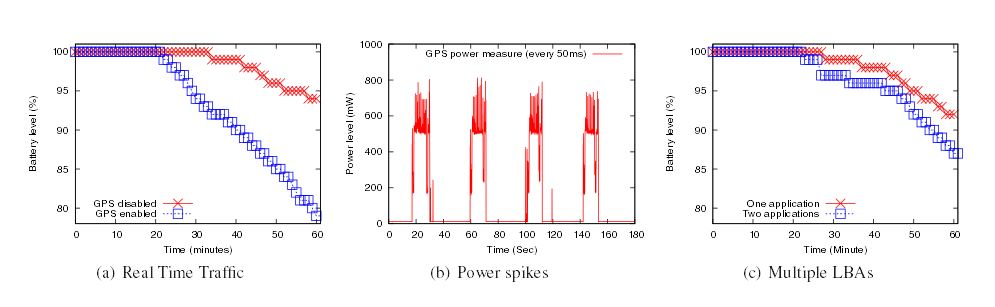
\includegraphics[scale=.5]{efficient}
\caption{\label{fig:efficient} Battery life based on tested parameters.}
\end{center}
\end{figure}

In the research, the authors were able to significantly improve battery life in several ways. By substituting a call for the GPS function, it was able to provide data that was acquired a short time ago. Though this will introduce a small amount of error in the readings, because the calls were so close it was insignificant. Most notably, the authors suppressed the GPS calls or piggybacked them. This result is very applicable to the proposed research as it can be used for not only location information prioritization, but can be implemented to manage data transmission. The authors found a large drop in battery life by turning on the GPS, and having several applications accessing it at once as seen in figure \ref{fig:efficient}.

\begin{figure}
\begin{center}
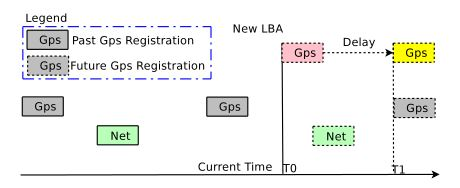
\includegraphics[scale=.8]{hold}
\caption{\label{fig:hold} Piggyback method postpones one call and synchronizes with others to cut calls to GPS unit.}
\end{center}
\end{figure}

In order to piggyback calls to the GPS, the authors decided to delay one call long enough that another is made. By doing this, the response time of the app suffers, but the power costs of turning the GPS on and off are negated. The method used to piggyback was actually very well implemented. The installed software monitors GPS usage for the apps and records patterns and access intervals. Using this method, the program is able to predict a call to the location unit. Using this information the program will postpone enabling the unit until another call has been made. At this point the GPS request will go through and the value returned from the hardware will be sent to both pieces of requesting software. This process can be seen in figure \ref{fig:hold}.

\begin{figure}
\begin{center}
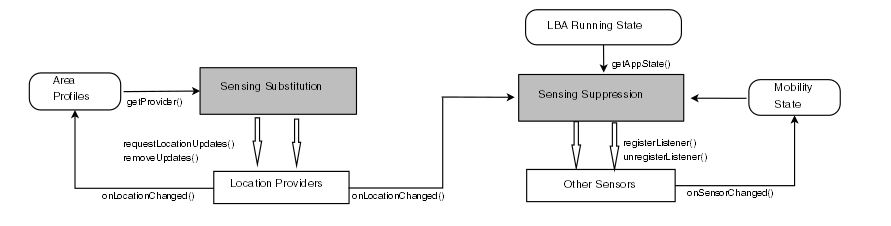
\includegraphics[scale=.6]{stop}
\caption{\label{fig:stop} The suppression method stops a call based on certain criteria.}
\end{center}
\end{figure}

In addition to the piggyback method, the suppression method described could be used to implement more efficient data transfer using the criteria described with minor modifications. The authors use an algorithm that checks the gyroscopes for movement and the screen for activity once per minute as seen in figure \ref{fig:stop}. If the device is not in motion, the GPS unit will turn off. By using this method with non cellular radios and other integrated devices the battery life of the device can be significantly improved.

In addition to to the research paper previously mentioned, additional research was completed with the goal of creating an energy \-aware framework for mobile platforms that monitors program activity and still retains usability. \cite{Fei:2008:EFD:1347375.1347380}. The writers were able to create a system that improved battery life with minimal impact to usability. Overall the authors methods could be implemented and used in the proposed research project, but the methods are very in depth and were shown to cause usability issues in some instances. The most valuable techniques that could be used are the power measurement methods and the evaluation methods.

\vspace*{-.2in}
\section{Method of Approach}
\label{sec:method}
\vspace*{-.1in}

The proposed research will require both hardware and software modifications. To begin, the project will implement a variant of the program designed by the researchers trying to improve battery life by reducing calls to the GPS unit. In addition to the software, voltage and current monitoring hardware will need to be implemented so energy efficiency results can be gathered.

The software variant will implement several familiar features. These features will include data and GPS call piggybacking, suppression, and optimization. For data piggybacking, all calls to the GPS will be handled as they were in the previous paper. \cite{Zhuang:2010:IEE:1814433.1814464} In order to reduce the number of data send and receiving calls a queue will be implemented to hold data calls. Once a request delay passes the queue will be executed until all calls have been completed. The delay will be automatically determined by the software after monitoring trends and user activity. When the device is locked and no longer in use, any programs that do not require constant data connection such as phone, messaging, and email, the apps will be placed into a state of sleep where data requests will be queued. Once the phone is activated these backlogs will be executed from the latest request to the oldest to ensure optimal response time.

Lastly, the mobile data connections will be optimized based on connection speeds. Connections with a faster transfer rate will be favored, making the time necessary for the device to be actively sending and receiving data minimized as much as possible. If one connection has an excessive number of connection requests another can be utilized if available.

\vspace*{-.2in}
\section{Evaluation Strategy}
\label{sec:evaluate}
\vspace*{-.1in}

Evaluating the effectiveness of the program is relatively straightforward and will be monitored for each of four variables. To be able to monitor energy efficiency, the device will be hooked up to a power monitoring device similar to the one in figure \ref{fig:power}. This set up will be used to gather a base reading for voltage and amperage of the device running the included weather app and a reading of the phone in a locked state. With the device in factory condition a fully charged battery will be timed until the phone shuts off. The device will be used for three hours browsing internet, and the remaining time will be spent in locked mode. The last baseline parameter would gauge any visible lags in performance when the user is actively interacting with the device.

\begin{figure}
\begin{center}
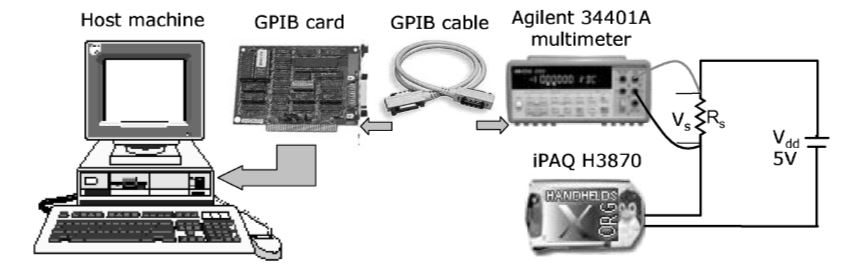
\includegraphics[scale=.6]{power}
\caption{\label{fig:power} Power measurement setup used by previous researchers \cite{Fei:2008:EFD:1347375.1347380}}
\end{center}
\end{figure}

Again, the same tests will be performed, but will be run with the proposed program. A computer will record voltage and amperage. Battery life will be timed by running a stopwatch in the background and when the phone shuts off the state of the watch will halt and will be recorded. Usability, as before, will be determined by the user.

\vspace*{-.1in}
\section{Research Schedule}
\label{sec:schedule}
\vspace*{-.1in}

To begin the project several topics must be addressed, namely development, implementation, and testing of the proposed systems and programs. 

Phase 1 - 1 week: Research and obtain hardware necessary to record baseline recordings.

Phase 2 - 2-3 months: Develop a working program which is capable of satisfying the requirements outlined in section \ref{sec:method}. Take baseline readings before program is installed. Install program and test for stability.

Phase 3 - 1 week: During this time I will run various tests on the program using the proposed methods in section \ref{sec:method} and record the results.

Phase 4 - remaining time: The results gathered throughout the test process will be evaluated and the software tweaked and finalized. After modifications are complete tests will be rerun and the final results will be evaluated.

\vspace*{-.1in}
\section{Conclusion}
\label{sec:conclusion}
\vspace*{-.1in}

Mobile devices are becoming more prominent in most people's daily lives -- to the point of individuals becoming reliant on the availability of the devices. This raises a need for more energy efficient devices that require less charge time and more time actively being used. In order to do this manufacturers have implemented sensors to adjust screen brightness and other hardware settings to improve this. Software can play a massive role in power usage, and in many cases is the culprit for most consumption. By reducing the number and frequency of calls to GPS and data transfer hardware and allowing connections and apps to be optimized and put to sleep can drastically improve not only battery life, but user experience.

\bibliographystyle{plain}
\bibliography{senior_thesis_proposal}

\end{document}

